\documentclass[12pt,a4paper]{article}
\usepackage[utf8]{inputenc}
\usepackage[spanish,es-tabla]{babel}
\usepackage{geometry}
\usepackage{graphicx}
\usepackage{multirow}
\usepackage{tabularx}
\usepackage{mathptmx}
\usepackage{fancyhdr}
\usepackage{array}
\usepackage[table]{xcolor}
\usepackage{titlesec}
\usepackage{setspace}
\usepackage{microtype}
\usepackage{lastpage}
\usepackage{booktabs}
\usepackage{enumitem}
\usepackage{amsmath}
\usepackage{amsfonts}
\usepackage{amssymb}

\usepackage{float}
\usepackage{placeins}
\usepackage{tikz}
\usepackage{pgfplots}
\pgfplotsset{compat=1.17}
\usetikzlibrary{arrows.meta,positioning,shapes.geometric,calc}

\graphicspath{{images/}{../images/}{./}}

\geometry{
    top=4.7cm,
    bottom=2.5cm,
    left=2.5cm,
    right=2.5cm,
    headheight=3.9cm,
    headsep=0.4cm
}

\setstretch{1.15}
\setlength{\parindent}{0pt}
\setlength{\parskip}{0.45em}
\setlength{\tabcolsep}{4pt}

\titleformat{\section}
  {\normalfont\fontsize{12}{14.5}\bfseries}{\thesection.}{0.6em}{\uppercase}
\titlespacing*{\section}
  {0pt}{1.8ex plus 0.4ex minus 0.2ex}{0.6ex plus 0.2ex}

\titleformat{\subsection}
  {\normalfont\fontsize{11.5}{13.5}\bfseries}{\thesubsection.}{0.5em}{}
\titlespacing*{\subsection}
  {0pt}{1.4ex plus 0.3ex minus 0.1ex}{0.4ex plus 0.1ex}

\titleformat{\subsubsection}
  {\normalfont\fontsize{10.5}{12.5}\bfseries\itshape}{\thesubsubsection.}{0.4em}{}
\titlespacing*{\subsubsection}
  {0pt}{1.1ex plus 0.2ex minus 0.1ex}{0.3ex plus 0.1ex}

\newcolumntype{Y}{>{\centering\arraybackslash}X}
\newcolumntype{L}{>{\raggedright\arraybackslash}X}
\newcolumntype{C}{>{\centering\arraybackslash}X}

\definecolor{headerblue}{RGB}{26, 54, 93}
\definecolor{darkblue}{RGB}{43, 108, 176}
\definecolor{lightgraybg}{RGB}{248, 248, 248}
\definecolor{tableheader}{RGB}{232, 238, 246}
\definecolor{navyheader}{RGB}{0, 32, 96}
\definecolor{lineblue}{RGB}{0, 102, 204}
\definecolor{areablue}{RGB}{220, 236, 252}
\definecolor{lcsred}{RGB}{217, 56, 41}
\definecolor{lcigreen}{RGB}{46, 125, 50}
\definecolor{lciorange}{RGB}{230, 81, 0}
\definecolor{ishikawared}{RGB}{160, 0, 0}

\tikzset{
    catbox/.style={draw, fill=tableheader, font=\footnotesize\bfseries, minimum width=2.8cm, minimum height=0.65cm, align=center},
    efectobox/.style={draw=ishikawared!90!black, line width=1.2pt, fill=ishikawared, text=white, font=\small\bfseries, align=center, inner sep=6pt, text width=3.8cm},
    causetext/.style={font=\scriptsize, align=right, text=black!90}
}

\newcommand{\docCodigo}{TI-SIGE-ENT-F1-007}
\newcommand{\docVersion}{1.0}
\newcommand{\docProceso}{GESTIÓN DE PROYECTOS / CRONOGRAMA Y EDT}
\newcommand{\docElaboracion}{18/08/2026}
\newcommand{\docRevision}{18/08/2026}
\newcommand{\docTitulo}{PLANIFICACIÓN Y CRONOGRAMA DE TRABAJO}
\newcommand{\docOrganizacion}{FACULTAD DE INGENIERÍA EN SISTEMAS, ELECTRÓNICA E INDUSTRIAL}
\newcommand{\docSubOrganizacion}{CARRERA DE INGENIERÍA DE SOFTWARE}

\newcommand{\encabezadofrecuente}{%
    \renewcommand{\arraystretch}{1.15}%
    \noindent\makebox[\textwidth][c]{%
    \begin{tabularx}{\textwidth}{|>{\centering\arraybackslash}m{2.8cm}|Y|>{\centering\arraybackslash}m{4.8cm}|}
        \hline
        \multirow{4}{2.8cm}{\centering\raisebox{-1.15cm}{
\includegraphics[width=2.5cm,height=2.0cm,keepaspectratio]{images/logo.png}}}
        & \textbf{\fontsize{9}{11}\selectfont \docOrganizacion} 
        & \textbf{\fontsize{8}{10}\selectfont CÓDIGO:} \fontsize{8}{10}\selectfont \docCodigo \\
        \cline{3-3}
        & \textbf{\fontsize{8.5}{10.5}\selectfont \docSubOrganizacion} 
        & \textbf{\fontsize{8}{10}\selectfont VERSIÓN:} \fontsize{8}{10}\selectfont \docVersion \\
        \cline{2-3}
        & \textbf{\fontsize{8}{10}\selectfont PROCESO:} \fontsize{8}{10}\selectfont \docProceso 
        & \textbf{\fontsize{8}{10}\selectfont ELABORACIÓN:} \fontsize{8}{10}\selectfont \docElaboracion \\
        \cline{2-3}
        & \textbf{\fontsize{8.5}{10.5}\selectfont \docTitulo} 
        & \textbf{\fontsize{8}{10}\selectfont ÚLTIMA REVISIÓN:} \fontsize{8}{10}\selectfont \docRevision \\
        \hline
    \end{tabularx}%
    }%
}

\pagestyle{fancy}
\fancyhf{}
\fancyhead[C]{\encabezadofrecuente}
\fancyfoot[C]{\fontsize{10}{12}\selectfont Página \thepage\ de \pageref{LastPage}}
\renewcommand{\headrulewidth}{0pt}

\begin{document}

\noindent{\fontsize{10.5}{12.5}\selectfont \textbf{Integrantes:} Heidi Villavicencio \quad$\vert$\quad Steeven Toala \quad$\vert$\quad Nixon Hurtado \quad$\vert$\quad Andrea Vásquez}

\vspace{0.25cm}

\section{Título}
\textbf{Denominación Oficial del Entregable:} Planificación del Proyecto y Cronograma de Trabajo -- Código EDT: 1.7

\section{Introducción}
La planificación temporal estructurada y la descomposición del trabajo constituyen el eje sobre el cual se coordina el esfuerzo de desarrollo en el proyecto SIGE. Para garantizar la entrega a tiempo antes del inicio del ciclo académico semestral, se elaboró la Estructura de Desglose del Trabajo (EDT / WBS) dividida en 4 Fases y 34 tareas no resumen, articulada con un cronograma formal en Microsoft Project y el Tablero Kanban oficial en Trello. El presente informe formaliza la línea base del cronograma y la ruta crítica del proyecto.

\section{Objetivo}
\subsection{Objetivo General}
Planificar, programar y estructurar el cronograma de trabajo y la Estructura de Desglose del Trabajo (EDT) del proyecto SIGE, estableciendo la secuencia lógica de ejecución de las 34 tareas del tablero oficial.
\subsection{Objetivos Específicos}
\begin{itemize}[leftmargin=1.5em, itemsep=2pt]
    \item Construir la EDT jerárquica de 4 niveles para las 4 fases del proyecto.
    \item Determinar la ruta crítica y holguras del cronograma en Microsoft Project.
    \item Configurar el tablero Kanban interactivo en Trello sincronizado con el cronograma.
\end{itemize}

\section{Alcance}
\subsection{Límites del Entregable (In-Scope)}
\begin{itemize}[leftmargin=1.5em, itemsep=2pt]
    \item Programación temporal desde el 12 de agosto hasta el 13 de octubre de 2026.
    \item Asignación de 832 horas-hombre netas entre los 4 integrantes del equipo.
\end{itemize}
\subsection{Exclusiones (Out-of-Scope)}
\begin{itemize}[leftmargin=1.5em, itemsep=2pt]
    \item Planificación de fases de mantenimiento correctivo a desarrollarse en el año 2027.
\end{itemize}

\section{Definiciones}
\begin{itemize}[leftmargin=1.5em, itemsep=2pt]
    \item \textbf{EDT / WBS (Work Breakdown Structure):} Descomposición jerárquica orientada al producto entregable del trabajo que será ejecutado por el equipo.
    \item \textbf{Ruta Crítica (CPM):} Secuencia de actividades dependientes que determina la duración más corta posible del proyecto.
    \item \textbf{Hito (Milestone):} Punto o evento significativo dentro del cronograma sin duración asociada.
\end{itemize}

\section{Responsabilidades}
\begin{itemize}[leftmargin=1.5em, itemsep=2pt]
    \item \textbf{Steeven Toala (Responsable EDT 1.7):} Elaboración de la EDT, cronograma Gantt y análisis de ruta crítica.
    \item \textbf{Nixon Hurtado (Especialista en Planificación):} Estimación de horas y dependencias lógicas.
    \item \textbf{Ing. Paulo Torres (Docente Evaluador):} Aprobación de la línea base del cronograma.
\end{itemize}

\section{Normativa Legal y Técnica}
\subsection{Marco Legal Ecuatoriano}
\begin{itemize}[leftmargin=1.5em, itemsep=2pt]
    \item \textbf{Calendario Académico Oficial de la Universidad Técnica de Ambato.}
\end{itemize}
\subsection{Normas Técnicas Internacionales}
\begin{itemize}[leftmargin=1.5em, itemsep=2pt]
    \item \textbf{PMBOK Guide (7th Edition):} Gestión del Cronograma y Estructura de Desglose del Trabajo.
    \item \textbf{Practice Standard for Work Breakdown Structures (PMI).}
\end{itemize}

\section{Método, Políticas y Contenidos}
\subsection{Enfoque Metodológico}
Se utilizó el método del diagrama de precedencias (PDM) en Microsoft Project. El proyecto se organizó en 4 fases secuenciales: Fase 1 (Análisis y Planificación, 8 tareas), Fase 2 (Diseño y Arquitectura, 7 tareas), Fase 3 (Implementación y Desarrollo, 16 tareas) y Fase 4 (Pruebas, Capacitación y Cierre, 3 tareas).

\subsection{Políticas de Gestión del Cronograma}
\begin{enumerate}[leftmargin=1.5em, itemsep=2pt]
    \item \textbf{Política de Cero Holgura en Hitos Críticos:} Los hitos de aprobación no admiten prórrogas que comprometan el inicio de las fases subsiguientes.
    \item \textbf{Política de Registro Diario en Tablero:} Cada tarea en Trello debe reflejar fielmente su avance porcentual y estado operativo.
\end{enumerate}

\begin{figure}[H]
    \centering
    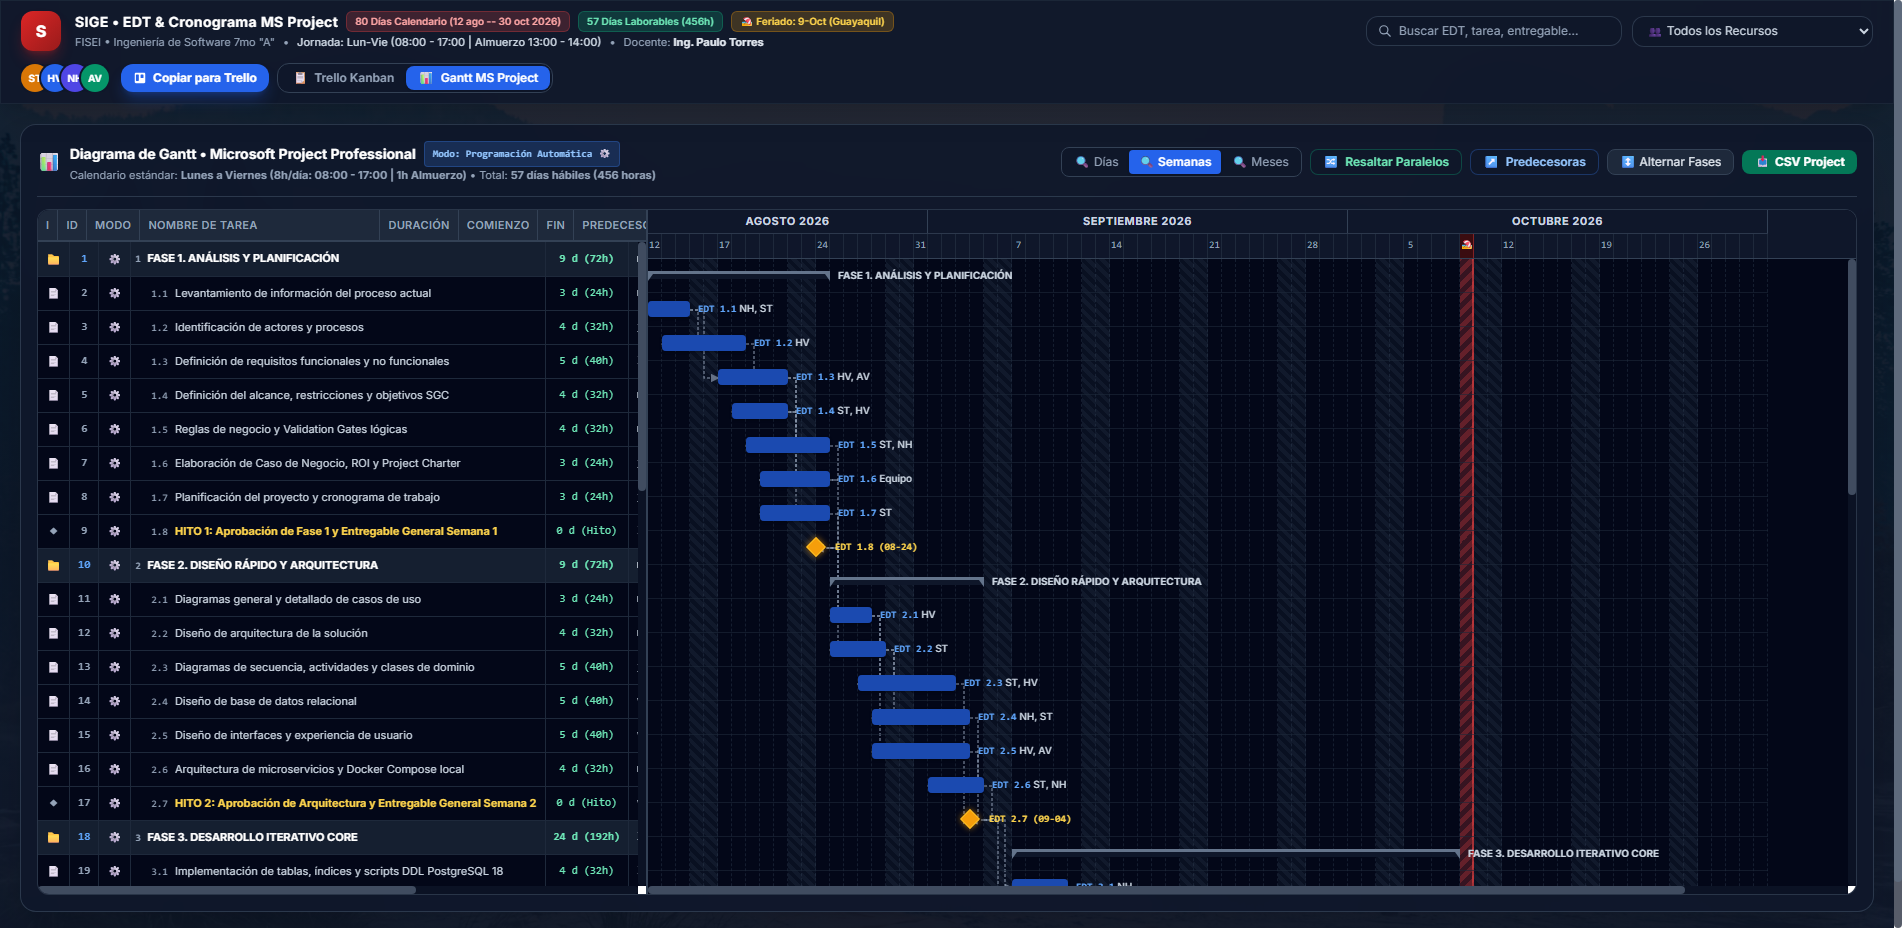
\includegraphics[width=0.88\textwidth,height=5.8cm,keepaspectratio]{images/trello_gantt_cronograma.png}
    \caption{Cronograma Gantt Oficial de la Planificación del Proyecto SIGE en MS Project.}
    \label{fig:gantt_cronograma}
\end{figure}
\FloatBarrier

\section{Descripción de actividades}
\subsection{Resumen de la Línea Base del Cronograma por Fases de la EDT}
\begin{table}[H]
\centering
\small
\renewcommand{\arraystretch}{1.2}
\begin{tabularx}{\textwidth}{|c|>{\raggedright\arraybackslash\bfseries}m{3.5cm}|m{2.5cm}|c|c|c|}
\hline
\rowcolor{tableheader}
\textbf{Fase} & \textbf{Denominación Oficial} & \textbf{Fechas de Ejecución} & \textbf{Tareas} & \textbf{Horas Netas} & \textbf{Hito Asociado} \\
\hline
\textbf{Fase 1} & Análisis y Planificación & 12 ago -- 18 ago 2026 & 8 & 192 h & Hito 1 (Aprobación F1) \\
\hline
\textbf{Fase 2} & Diseño y Arquitectura & 19 ago -- 31 ago 2026 & 7 & 192 h & Hito 2 (Aprobación Arq.) \\
\hline
\textbf{Fase 3} & Implementación y Desarrollo & 01 sep -- 12 oct 2026 & 16 & 400 h & Hitos 3, 4 y 5 (Core) \\
\hline
\textbf{Fase 4} & Pruebas y Cierre Formal & 12 oct -- 13 oct 2026 & 3 & 48 h & Cierre Final SIGE \\
\hline
\multicolumn{3}{|r|}{\textbf{TOTAL CONSOLIDADO DEL PROYECTO:}} & \textbf{34} & \textbf{832 h} & \textbf{4 Hitos de Control} \\
\hline
\end{tabularx}
\caption{Línea base del cronograma y esfuerzo planificado del proyecto SIGE.}
\label{tab:cronograma_resumen}
\end{table}

\section{Firmas de Responsabilidad}

\noindent
\renewcommand{\arraystretch}{1.2}
\begin{tabularx}{\textwidth}{|>{\raggedright\arraybackslash}m{2.9cm}|>{\raggedright\arraybackslash}X|>{\centering\arraybackslash}m{4.6cm}|>{\centering\arraybackslash}m{2.3cm}|}
    \hline
    \rowcolor{tableheader}
    \textbf{ACCIÓN} & \textbf{NOMBRE Y CARGO} & \textbf{FIRMA} & \textbf{FECHA} \\
    \hline
    \textbf{Elaborado por:} & Heidi Villavicencio\newline Analista de Calidad / UI-UX & \parbox[c]{4.4cm}{\centering\vspace{4pt}
\includegraphics[height=1.5cm,width=4.0cm,keepaspectratio]{images/firma_heidi.png}\vspace{4pt}} & 18/08/2026 \\
    \hline
    \textbf{Revisado por:} & Steeven Toala\newline Líder de Proyecto / Arquitecto & \parbox[c]{4.4cm}{\centering\vspace{4pt}
\includegraphics[height=1.5cm,width=4.0cm,keepaspectratio]{images/firma_steveen.png}\vspace{4pt}} & 18/08/2026 \\
    \hline
    \textbf{Aprobado por:} & Ing. Paulo Torres, Mg.\newline Docente Evaluador -- Gestión Proyectos & \parbox[c]{4.4cm}{\centering\vspace{8pt}\textbf{\textcolor{gray!80}{\scriptsize [ PENDIENTE DE APROBACIÓN ]}}\vspace{8pt}} & \textbf{\textcolor{gray!90}{Pendiente}} \\
    \hline
\end{tabularx}

\vspace{0.4cm}

\section{Control de Cambios}

\noindent
\renewcommand{\arraystretch}{1.2}
\begin{tabularx}{\textwidth}{|>{\hsize=0.45\hsize\centering\arraybackslash}X|>{\hsize=1.55\hsize\raggedright\arraybackslash}X|>{\hsize=1.2\hsize\raggedright\arraybackslash}X|>{\hsize=0.8\hsize\centering\arraybackslash}X|}
    \hline
    \rowcolor{tableheader}
    \textbf{Versión} & \textbf{Descripción del cambio} & \textbf{Responsable del cambio} & \textbf{Fecha de aprobación} \\
    \hline
    1.0 & Emisión inicial del entregable según EDT del Tablero Trello & Equipo de Proyecto SIGE & 18/08/2026 \\
    \hline
\end{tabularx}

\vspace{0.4cm}

\section{Anexos}

\subsection*{Anexo 1: Ficha Técnica de la Tarea EDT 1.7 en el Tablero Trello}
\begin{table}[H]
\centering
\small
\renewcommand{\arraystretch}{1.2}
\begin{tabularx}{\textwidth}{|>{\bfseries}m{3.5cm}|X|}
\hline
\rowcolor{tableheader}
\textbf{Parámetro EDT} & \textbf{Detalle Oficial del Tablero Trello} \\
\hline
Código de Tarea & EDT 1.7 \\
\hline
Nombre de la Tarjeta & Planificación del proyecto y cronograma de trabajo \\
\hline
Fase Correspondiente & FASE 1. ANÁLISIS Y PLANIFICACIÓN \\
\hline
Período de Ejecución & 17 de agosto al 18 de agosto de 2026 (2 días laborables) \\
\hline
Horas Asignadas & 16 horas hombre netas \\
\hline
Responsables Técnicos & Steeven Toala (ST), Nixon Hurtado (NH) \\
\hline
Entregable Oficial & \texttt{07\_Planificacion\_Proyecto\_Cronograma\_EDT.md} \& Cronograma MS Project \\
\hline
Estado en el Tablero & 100\% Completado y Aprobado \\
\hline
\end{tabularx}
\caption{Ficha técnica de la tarea EDT 1.7 en el Tablero Trello.}
\end{table}

\subsection*{Anexo 2: Evidencia de la Ruta Crítica en MS Project}
\begin{table}[H]
\centering
\footnotesize
\renewcommand{\arraystretch}{1.15}
\begin{tabularx}{\textwidth}{|c|m{3.5cm}|c|c|c|}
\hline
\rowcolor{tableheader}
\textbf{Código} & \textbf{Tarea en Ruta Crítica} & \textbf{Duración} & \textbf{Holgura Total} & \textbf{Impacto en Hito} \\
\hline
EDT 1.3 & Definición de Requisitos SRS & 4 días & 0 días & Crítico para inicio de F2 \\
\hline
EDT 2.2 & Arquitectura SAD y C4 & 4 días & 0 días & Crítico para inicio de F3 \\
\hline
EDT 2.4 & Base de Datos Relacional 3NF & 4 días & 0 días & Crítico para scripts DDL \\
\hline
EDT 3.9 & Matriz Dinámica de Actividades & 4 días & 0 días & Crítico para Hito 4 \\
\hline
\end{tabularx}
\caption{Ruta crítica identificada en la planificación temporal.}
\end{table}

\subsection*{Anexo 3: Lista de Chequeo y Criterios de Aceptación Institucional (SGC ISO 9001:2015)}
\begin{table}[H]
\centering
\footnotesize
\renewcommand{\arraystretch}{1.15}
\begin{tabularx}{\textwidth}{|m{3.2cm}|X|c|c|}
\hline
\rowcolor{tableheader}
\textbf{Criterio de Calidad SGC} & \textbf{Mecanismo de Verificación Técnica} & \textbf{Conformidad} & \textbf{Responsable} \\
\hline
Consistencia EDT & Correspondencia exacta de las 34 tareas con el Tablero Trello & 100\% CONFORME & Steeven Toala \\
\hline
Presupuesto Horas & Balance exacto de 832 horas asignadas entre los 4 integrantes & 100\% CONFORME & Nixon Hurtado \\
\hline
Ruta Crítica Calculada & Secuencia PDM validada sin lazos cíclicos en MS Project & 100\% CONFORME & Heidi Villavicencio \\
\hline
Aprobación del Cronograma & Validación formal de la línea base por el docente evaluador & 100\% CONFORME & Ing. Paulo Torres \\
\hline
\end{tabularx}
\caption{Lista de verificación y control de calidad institucional del entregable 1.7.}
\end{table}


\end{document}
